\section{Serveur Web intégré}

\subsection{Avantages}
\begin{frame}
	\frametitle{Serveur web intégré}
	\framesubtitle{Avantages de la solution}
	\begin{itemize}
		\item Dépendances du projet réduites au strict minimum
			\begin{itemize}
				\item Installation sur système minimal
				\item Pas de configurations
				\item Portabilité et rapidité de déploiement
			\end{itemize}
		\item Serveur minimaliste = moins de code = moins de failles
			\begin{itemize}
				\item Réponse a des requêtes précises
				\item Peu de fonctionnalités : inutile d'ouvrir trop
				\item Taille réduite (Apache : 10Mo, octoBrain : 220Ko)
			\end{itemize}
	\end{itemize}
\end{frame}

\subsection{Conception}
\begin{frame}
	\frametitle{Serveur web intégré}
	\framesubtitle{Choix de conception}
	\begin{itemize}
		\item Uniquement requête GET
		\item Deux fonctionnements : fichiers ou service
		\item Envoi de fichiers au début, puis AJAX uniquement
		\item Single-thread
		\item HTTPS Only
	\end{itemize}
\end{frame}

\subsection{Résultat}
\begin{frame}
	\frametitle{Serveur web intégré}
	\framesubtitle{Exemple du résultat}
	\begin{figure}[!h]
		\begin{center}
			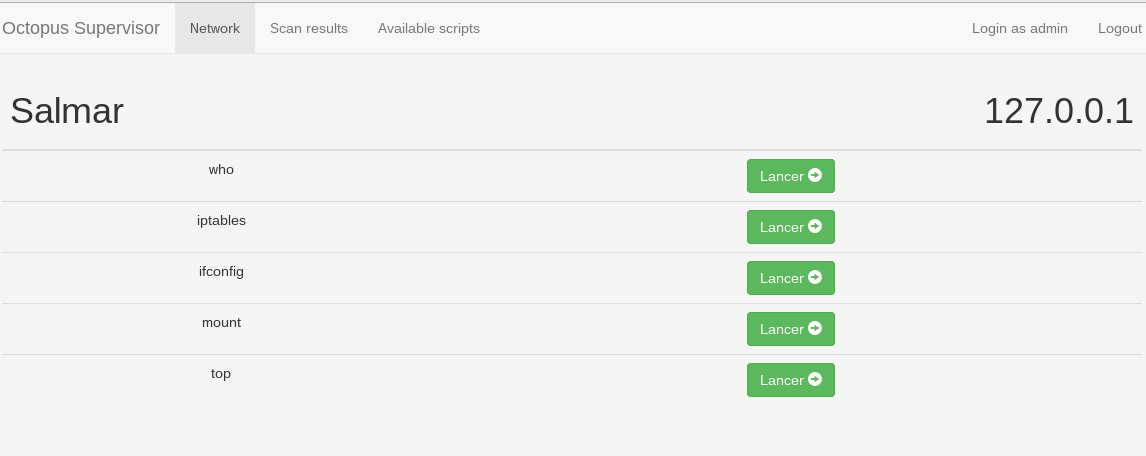
\includegraphics[width=\textwidth]{images/screen_web.png}
		\end{center}
	\end{figure}
\end{frame}
\begin{frame}[fragile]
	\frametitle{Serveur web intégré}
	\framesubtitle{Exemple du résultat}
	https://localhost:8080/service?
	   action=gettentacles\&key=560121136\&id=2
	\begin{minted}[tabsize=3,
			frame=lines,
			framesep=2mm,
			linenos,
		startinline]{json}
		{
		 "success":true,
		 "tentacles":[
		  {
		   "id":506138912,
		   "hostname":"Salmar",
		   "ip":"127.0.0.1",
		   "lastalive":1423679166
		  }
		 ]
		}
	\end{minted} 
\end{frame}

\section{Maestro}
\subsection{Avantages}
\begin{frame}
	\frametitle{Maestro}
	\framesubtitle{Avantages de ce daemon}
	\begin{itemize}
		\item Point central du serveur
		\item Accès unique à la Base de Données
		\item Un point central à sécuriser
	\end{itemize}
\end{frame}

\subsection{Conception}
\begin{frame}
	\frametitle{Maestro}
	\framesubtitle{Conception}
	\begin{itemize}
		\item Création des pipes pour chaque fork : WebServ, registerer et commander
		\item Interprétation des commandes reçues sur les différents pipes
		\item Interaction avec les fonctions de lecture et écriture de la BDD
		\item Envoi des réponses au pipe correspondant
	\end{itemize}
	\begin{figure}
	    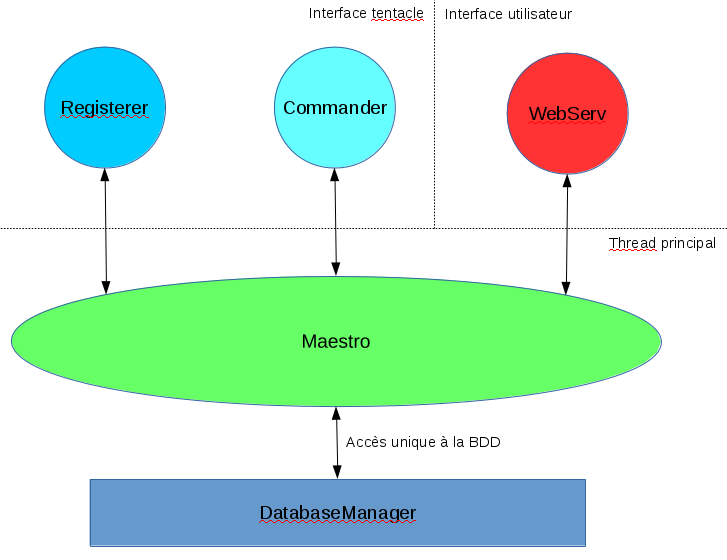
\includegraphics[height=3cm, keepaspectratio=true]{../rapport_octopus/img/algo_brain_full.png}
	\end{figure}
\end{frame}

\subsection{Résultat}
\begin{frame}[fragile]
	\frametitle{Maestro}
	\framesubtitle{Résultat}
	\begin{itemize}
		\item Select pipe
	\end{itemize}
	\begin{minted}[tabsize=3,
			frame=lines,
			framesep=2mm,
			linenos,
		startinline,
		fontsize=\tiny]{c}
		while(select(maxfd+1, &rfds, NULL, NULL, NULL) != -1){
		   logError(LOG_LEVEL_DEBUG,"maestro:maestro_start : select got data.");
		   if(FD_ISSET(webServ_speak_pipe[0],&rfds)){
		       ...
		       readLen = read(webServ_speak_pipe[0],bufIn,BUFSIZ);
		       ...
		       interpret_msg(bufIn,webServ_listen_pipe[1]);
		   }
		   if(FD_ISSET(registerer_speak_pipe[0],&rfds)){
		      ...
		      readLen = read(registerer_speak_pipe[0],bufIn,BUFSIZ);
		      ...
		      interpret_msg(bufIn,registerer_listen_pipe[1]);
		   }
		   if(FD_ISSET(cmd_speak_pipe[0], &rfds)){
		       do { read(...) }while;
		       ...
		       interpret_msg(buffer, cmd_listen_pipe[1]);
		  }

	\end{minted} 

\end{frame}

\section{Questions}
\begin{frame}
	\frametitle{Questions}
	\framesubtitle{Avez-vous des questions ?}
	Merci pour votre écoute.
	\newline
	Avez-vous des questions ?
\end{frame}

